\section{Proof by induction}
หากจะมองกลับไปเมื่อเรานิยามจำนวนนับ (natural numbers) ด้วยวิธีอุปนัย เราสามารถเขียน inference rule ได้ดังนี้
\[
\inferrule*[Right=nat-ind]
{\Gamma\vdash P(0) \\ \Gamma\vdash\forall n:P(n)\implies P(\mathrm{succ}(n))}
{\Gamma\vdash\forall n: P(n)}
\]
แต่เราทราบดีว่า จำนวนนับนั้นก็คือเซต $\mathbb{N}$ \enskip เราจึงสามารถเปลี่ยน $\mathrm{nat}$ ให้เป็น $\mathbb{N}$ และเปลี่ยน $\mathrm{succ}$ ให้เป็นการบวกเพิ่มด้วย 1 ทำให้ได้ inference rule ใหม่ดังนี้
\[
\inferrule*[Right=$\mathbb{N}$-ind]
{\Gamma\vdash P(0) \\ \Gamma\vdash\forall n:P(n)\implies P(n+1)}
{\Gamma\vdash\forall n: P(n)}
\]
ซึ่งเป็นที่มาของวิธีการพิสูจน์โดยอุปนัย ดังที่จะได้กล่าวต่อไป

\emph{การพิสูจน์โดยอุปนัย} (proof by induction) เป็นกลวิธีที่ใช้ในการพิสูจน์ว่า predicate $P(n)$ นั้นเป็นจริงสำหรับจำนวนนับ $n$ ทุกตัว โดยใช้ axiom เพื่อแบ่งขั้นตอนการพิสูจน์ออกเป็น 2 ขั้นตอนย่อยๆ ด้วยกัน ได้แก่ ขั้นฐาน และขั้นอุปนัย

Axiom ที่จะใช้ในการพิสูจน์ มีดังนี้
\begin{axiom}[induction]
ให้ $P(n)$ เป็น predicate โดยที่ $n\in\mathbb{N}$ \enskip ถ้าสองเงื่อนไขต่อไปนี้เป็นจริง
\begin{enumerate}
\item $P(0)$ เป็นจริง และ
\item $\forall n\in\mathbb{N}:P(n)\implies P(n+1)$ เป็นจริง
\end{enumerate}
แล้ว $\forall n\in\mathbb{N}:P(n)$ จะเป็นจริงด้วย
\end{axiom}
นั่นคือ หากต้องการสรุปว่า $P(n)$ เป็นจริงสำหรับจำนวนนับ $n$ ทุกตัว ให้พิสูจน์สองสิ่งต่อไปนี้
\begin{enumerate}
\item $P(0)$ เป็นจริง
\item $P(n+1)$ จะเป็นจริงด้วย หากสมมุติว่า $P(n)$ นั้นเป็นจริง โดยที่ $n$ เป็นจำนวนนับใดๆ
\end{enumerate}
เมื่อพิสูจน์ทั้งสองสิ่งดังกล่าวได้แล้ว จะได้ว่า เงื่อนไขตั้งต้นทั้งสองของ induction axiom นั้นเป็นจริง ซึ่งทำให้เราสามารถสรุปได้ว่า $P(n)$ เป็นจริงสำหรับจำนวนนับ $n$ ทุกตัว

ดังนั้น ขั้นตอนการเขียนบทพิสูจน์โดยอุปนัย มีดังนี้
\begin{itemize}
\item By induction on $n$. (โดยที่ $n$ เป็นตัวแปรใน predicate $P$)
\item เขียน predicate $P(n)$ ที่จะใช้ใน induction axiom และในบทพิสูจน์
\item \emph{ขั้นฐาน} (base case): พิสูจน์ว่า $P(0)$ เป็นจริง
\item \emph{ขั้นอุปนัย} (inductive step): ตั้งสมมุติฐานว่า $P(n)$ เป็นจริง เพื่อใช้ในการพิสูจน์ว่า $P(n+1)$ เป็นจริง
\item ใช้ induction axiom เพื่อสรุปว่า $P(n)$ เป็นจริงสำหรับจำนวนนับ $n$ ทุกค่า
\end{itemize}

วิธีหนึ่งที่ช่วยให้เข้าใจการพิสูจน์โดยอุปนัยได้ดีขึ้น คือการมองเซตของจำนวนนับเป็นสายโดมิโนที่ยาวไปเรื่อยๆ ไม่สิ้นสุด กล่าวคือ $P(i)$ เปรียบเสมือนโดมิโนตัวที่ $i$ (โดยที่ $i$ เริ่มจาก $0$) และการที่ $P(i)$ เป็นจริง เปรียบเสมือนโดมิโนตัวที่ $i$ ล้ม \enskip Induction axiom นั้นกล่าวว่า หากต้องการจะสรุปว่าโดมิโนทุกตัวในสายยาวนี้ล้มทั้งหมด แค่หาหลักฐานสองอย่างต่อไปนี้ ก็เพียงพอที่จะสรุปได้
\begin{enumerate}
\item โดมิโนตัวที่ $0$ ล้ม และ
\item หากโดมิโนตัวที่ $i$ ล้ม แล้วโดมิโนตัวที่ $i+1$ จะล้มด้วย (ไม่ว่า $i$ จะเป็นจำนวนนับใดๆ ก็ตาม)
\end{enumerate}

\begin{theorem}\label{thm:sum-n}
ให้ $n\geq 0$
\[1+2+\cdots+n=\frac{n(n+1)}{2}\]

\noindent{\bf Remark}: ก่อนจะทำการพิสูจน์ ขอให้เข้าใจความหมายของ $\cdots$ ข้างต้นก่อน \enskip เราต้องหาแบบอย่าง (pattern) ให้ได้ว่า ส่วนที่ละไว้นั้นควรจะเป็นอะไร \enskip ในที่นี้ เป็นการบวกเลขตั้งแต่ $1$ ถึง $n$ ซึ่งแปลว่าหาก $n=2$ ก็คือ $1+2$ โดยไม่บวก $2$ ซ้ำสองครั้ง และหาก $n=0$ ก็คือเราต้องบวกเลขตั้งแต่ $1$ ถึง $0$ ซึ่งแปลว่าไม่มีเลขต้องบวก ดังนั้น ผลรวมก็ควรจะเป็น $0$
\begin{pf}
By induction on $n$.  ให้ $P(n)\triangleq 1+2+\cdots+n=\frac{n(n+1)}{2}$
\begin{itemize}
\item {\bf Base case}: ต้องพิสูจน์ว่า $P(0)$ เป็นจริง \enskip ทางด้านซ้ายของเครื่องหมาย $=$ เป็นผลบวกของเลขตั้งแต่ $1$ ถึง $0$ ซึ่งเป็นศูนย์ ส่วนทางด้านขวาของเครื่องหมาย $=$ นั้น $\frac{0(0+1)}{2}=0$ ด้วย \enskip ดังนั้น $P(0)$ เป็นจริง \quad\yea
\item {\bf Inductive step}: สมมุติว่า $P(n)$ เป็นจริง กล่าวคือ $1+2+\cdots+n=\frac{n(n+1)}{2}$ ต้องพิสูจน์ว่า \[1+2+\cdots+(n+1)=\frac{(n+1)(n+2)}{2}\] เมื่อแทนค่าจากสมมุติฐานและทำการจัดรูป จะได้ว่า
\begin{align*}
1+2+\cdots+(n+1)
&=\left[1+2+\cdots+n\right]+(n+1) \\
&=\frac{n(n+1)}{2}+(n+1) \qquad\textup{(by I.H.)} \\
&=(n+1)\left[\frac{n}{2}+1\right] \\
&=(n+1)\frac{n+2}{2}
\end{align*}
ตามที่ต้องการ \quad\yea
\end{itemize}
ดังนั้น จาก induction axiom จึงสรุปได้ว่า $1+2+\cdots+n=\frac{n(n+1)}{2}$ เมื่อ $n\geq 0$
\end{pf}
\end{theorem}

ถึงแม้ว่า induction axiom จะกล่าวว่าเราต้องเริ่ม base case จาก $n=0$ แต่ในความเป็นจริงแล้ว เราสามารถเริ่มจากจำนวนนับ (หรือแม้กระทั่งจำนวนเต็ม) ใดก็ได้ อย่างไรก็ดี ข้อสรุปจาก axiom ที่ตามมาก็ย่อมเปลี่ยนแปลงไปด้วย ตัวอย่างเช่น หากเริ่ม base case จาก $n=3$ เราจะสรุปได้เพียงแค่ $P(n)$ เป็นจริง เมื่อ $n\geq 3$ เท่านั้น หากเปรียบเทียบกรณีเหล่านี้กับสายโดมิโนอีกครั้งหนึ่ง จะได้ว่าเราเพิ่มหรือลดจำนวนโดมิโนที่อยู่หัวแถวนั่นเอง

\begin{theorem}
ผลรวมของจำนวนนับที่เป็นเลขคี่ $n$ ตัวแรก เท่ากับ $n^2$
\begin{pf}
By induction on $n$.  ให้ $P(n)\triangleq$ ผลรวมของจำนวนนับที่เป็นเลขคี่ $n$ ตัวแรก เท่ากับ $n^2$ (โดยที่ $n\geq 1$) \enskip เพื่อความสะดวกในการพิสูจน์ดังที่จะได้แสดง จะเขียน $P(n)$ โดยใช้สัญลักษณ์ทางคณิตศาสตร์ก่อน เนื่องจากจำนวนนับที่เป็นเลขคี่ตัวที่ $n$ มีค่าเท่ากับ $2n-1$ จะได้ว่า $P(n)\equiv 1+3+\cdots+(2n-1)=n^2$
\begin{itemize}
\item {\bf Base case}: ($n=1$) \quad ต้องพิสูจน์ว่า $P(1)$ เป็นจริง จะได้ว่า $1=1^2$ \quad\yea
\item {\bf Inductive step}: สมมุติว่า $P(n)$ เป็นจริง กล่าวคือ $1+3+\cdots+(2n-1)=n^2$ ต้องพิสูจน์ว่า \[1+3+\cdots+(2(n+1)-1)=(n+1)^2\] จะได้ว่า
\begin{align*}
1+3+\cdots+(2(n+1)-1)
&=\left[1+3+\cdots+(2n-1)\right]+(2(n+1)-1) \\
&=n^2+(2(n+1)-1) \qquad\textup{(by I.H.)} \\
&=n^2+2n+2-1 \\
&=n^2+2n+1 \\
&=(n+1)^2 \quad\textup{\yea}
\end{align*}
\end{itemize}
ดังนั้น ผลรวมของจำนวนนับที่เป็นเลขคี่ $n$ ตัวแรก เท่ากับ $n^2$ (เมื่อ $n\geq 1$)
\end{pf}
\end{theorem}

\begin{theorem}
$\forall n\in\mathbb{N}: 3\mid (4^n-1)$
\begin{pf}
By induction on $n$.  ให้ $P(n)\triangleq 3\mid(4^n-1)$
\begin{itemize}
\item {\bf Base case}: ($n=0$) \quad $4^0-1=0$ และ $3\mid 0$ ดังนั้น $P(0)$ เป็นจริง \quad\yea
\item {\bf Inductive step}: สมมุติว่า $3\mid (4^n-1)$ ต้องพิสูจน์ว่า $3\mid(4^{n+1}-1)$

เนื่องจาก $3\mid(4^n-1)$ (by I.H.) จะได้ว่ามี $k\in\mathbb{Z}$ ที่ทำให้ $4^n-1=3k$ \enskip ดังนั้น
\begin{align*}
4^{n+1}-1
&= 4(4^n)-1 \\
&= 4(4^n)-4+4-1 \\
&= 4(4^n-1)+3 \\
&= 4(3k)+3 \\
&= 3(4k+1)
\end{align*}
นั่นคือ $3\mid (4^{n+1}-1)$ ตามที่เราต้องการ \quad\yea
\end{itemize}
\end{pf}
\end{theorem}

นอกจาก induction จะใช้พิสูจน์สมการ (equations) ดังที่ได้เห็นในตัวอย่างข้างต้นแล้ว induction ยังสามารถใช้พิสูจน์อสมการ (inequalities) ได้อีกด้วย แต่มักจะต้องใช้เหตุผลที่บางครั้งอาจไม่ชัดแจ้งทันทีจากบทพิสูจน์ กล่าวอีกนัยหนึ่ง การพิสูจน์ inequalities โดยใช้ induction นั้นมักจะยากกว่าการพิสูจน์ equations \enskip อย่างไรก็ดี วิธีการและกลไกยังคล้ายเดิม คือ เราต้องแปลงรูป (rewrite) ฝั่งซ้ายของอสมการไปเป็นฝั่งขวาให้ได้ แต่แทนที่การแปลงแต่ละครั้งจะเท่ากัน เรามีตัวเลือกที่จะปรับค่าขึ้นหรือลงตามเครื่องหมายอสมการที่เราต้องการได้ ตัวอย่างเช่น
%
\begin{theorem}
$\forall n\in\mathbb{N}: 10^0+10^1+\cdots+10^n<10^{n+1}$
\begin{pf}
By induction on $n$.  ให้ $P(n)\triangleq 10^0+10^1+\cdots+10^n<10^{n+1}$
\begin{itemize}
\item {\bf Base case}: ($n=0$) \quad จะได้ว่า $10^0=1$ และ $10^{0+1}=10$ ดังนั้น $1<10$ \quad\yea
\item {\bf Inductive step}: สมมุติว่า $10^0+10^1+\cdots+10^n<10^{n+1}$ จะได้ว่า
\begin{align*}
10^0+10^1+\cdots+10^{n+1}
&=\left[10^0+10^1+\cdots+10^n\right]+10^{n+1} \\
&<10^{n+1}+10^{n+1} \qquad\textup{(by I.H.)} \\
&=2\cdot 10^{n+1} \\
&<10\cdot 10^{n+1} \qquad\textup{(เนื่องจาก $2<10$)} \\
&=10^{n+2}
\end{align*}
นั่นคือ $10^0+10^1+\cdots+10^{n+1}<10^{(n+1)+1}$ ดังนั้น $P(n+1)$ เป็นจริง \quad\yea
\end{itemize}
\end{pf}
\end{theorem}

\subsection{Problem solving using induction}

การพิสูจน์โดยอุปนัยในตัวอย่างที่ผ่านๆ มา อาจจะไม่เป็นที่น่าพอใจเท่าใดนัก เนื่องจากเราอาจจะต้องรู้คำตอบไว้ก่อนแล้วจึงค่อยมาพิสูจน์ความถูกต้องอีกครั้งหนึ่ง กล่าวคือ การพิสูจน์โดยอุปนัยดูเหมือนจะไม่ช่วยให้เราหาคำตอบได้ง่ายขึ้น \enskip ตัวอย่างเช่น
%ใน Theorem~\ref{thm:sum-n}
ในการพิสูจน์ผลลัพธ์ของการบวกเลขตั้งแต่ 1 ถึง $n$
\emph{สูตรในรูปแบบปิด} (closed-form formula) ที่ได้นั้นไม่ได้มาจากการพิสูจน์โดยอุปนัยแต่อย่างใด แต่เราต้องหาหรือเดาสูตรนี้มาก่อนเพื่อพิสูจน์ความถูกต้อง

อย่างไรก็ดี การพิสูจน์โดยอุปนัยสามารถใช้แก้ปัญหาบางประเภทได้ โดยได้ทั้งขั้นตอนวิธีการแก้ปัญหาและบทพิสูจน์ความถูกต้องในเวลาเดียวกัน ดังจะได้กล่าวต่อไป

สมมุติว่าเรามีสวนหย่อมขนาด $2^n\times 2^n$ ตารางหน่วย (โดยที่ $n\geq 0$) ที่เราต้องการเว้นที่ตรงกลางไว้ 1 ตารางหน่วยเพื่อตกแต่งด้วยรูปปั้น ดังรูปที่~\ref{fig:courtyard-2}
%
\begin{figure}
\centering
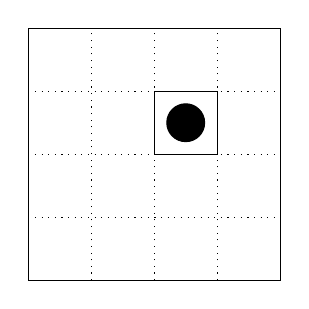
\begin{tikzpicture}[scale=0.8]
\draw[dotted] (0,0) grid (4,-4);
\draw (0,0) rectangle (4,-4);
\draw (2,-1) rectangle (3,-2);
\draw[fill] (2.5,-1.5) circle [radius=0.3cm];
\end{tikzpicture}
\caption{สวนหย่อมขนาด $2^n\times 2^n$ เมื่อ $n=2$ โดยเว้นช่องว่างไว้ให้รูปปั้นตรงกลาง}
\label{fig:courtyard-2}
\end{figure}
%
\enskip ในส่วนของพื้นที่ที่เหลือนั้น จะต้องปูกระเบื้องให้สวยงาม โดยที่กระเบื้องแต่ละชิ้นมีขนาด 3 ตารางหน่วย และมีรูปร่างคล้ายตัว L ดังรูปที่~\ref{fig:tile-shape}
%
\begin{figure}
\centering
\begin{tikzpicture}[scale=0.8]
\draw (0,0) -- (2,0) -- (2,-1) -- (1,-1) -- (1,-2) -- (0,-2) -- (0,0);
\draw[dotted] (1,0) -- (1,-1) -- (0,-1);
\end{tikzpicture}
\caption{รูปร่างของแผ่นกระเบื้องที่จะใช้ปูสวนหย่อม}
\label{fig:tile-shape}
\end{figure}
%
\enskip หาก $n=2$ เราอาจจะปูกระเบื้องได้ดังรูปที่~\ref{fig:courtyard-2-tiled}
%
\begin{figure}
\centering
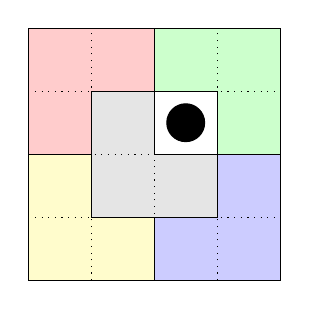
\begin{tikzpicture}[scale=0.8]
\draw[fill=red!20] (0,0) -- (2,0) -- (2,-1) -- (1,-1) -- (1,-2) -- (0,-2) -- (0,0);
\draw[fill=green!20] (2,0) -- (4,0) -- (4,-2) -- (3,-2) -- (3,-1) -- (2,-1) -- (2,0);
\draw[fill=blue!20] (4,-2) -- (4,-4) -- (2,-4) -- (2,-3) -- (3,-3) -- (3,-2) -- (4,-2);
\draw[fill=yellow!20] (0,-2) -- (0,-4) -- (2,-4) -- (2,-3) -- (1,-3) -- (1,-2) -- (0,-2);
\draw[fill=gray!20] (1,-1) -- (1,-3) -- (3,-3) -- (3,-2) -- (2,-2) -- (2,-1) -- (1,-1);

\draw[dotted] (0,0) grid (4,-4);
\draw[fill] (2.5,-1.5) circle [radius=0.3cm];
\end{tikzpicture}
\caption{วิธีการปูกระเบื้องบนสวนหย่อมในรูปที่~\ref{fig:courtyard-2}}
\label{fig:courtyard-2-tiled}
\end{figure}

ในตัวอย่างนี้ เราจะหาวิธีการปูกระเบื้องบนสวนหย่อมในลักษณะดังกล่าว รวมทั้งพิสูจน์ไปในตัวว่า วิธีการดังกล่าวนั้นถูกต้องไม่มีข้อผิดพลาด
%
\begin{theorem}
มีวิธีปูกระเบื้องรูปตัว L ลงบนสวนหย่อมขนาด $2^n\times 2^n$ ตารางหน่วย (เมื่อ $n\geq 0$) โดยเว้นช่องว่าง 1 ตารางหน่วยไว้ให้รูปปั้นตรงกลางสวนหย่อม
\begin{pf}[Failed proof]
By induction on $n$.  ให้ $P(n)\triangleq$ มีวิธีปูกระเบื้องรูปตัว L ลงบนสวนหย่อมขนาด $2^n\times 2^n$ โดยเว้นช่องว่าง 1 ตารางหน่วยไว้ให้รูปปั้นตรงกลางสวนหย่อม
\begin{itemize}
\item {\bf Base case}: ($n=0$) \quad ในกรณีนี้ สวนหย่อมมีขนาด $1\times 1$ ตารางหน่วย ซึ่งไม่เหลือพื้นที่ไว้ให้ปูกระเบื้อง ดังนั้น วิธีการปูกระเบื้องลงบนสวนหย่อมนี้ ก็คือการนั่งพักผ่อนอยู่เฉยๆ \quad\yea
\item {\bf Inductive step}: สมมุติว่ามีวิธีปูกระเบื้องรูปตัว L ลงบนสวนหย่อมขนาด $2^n\times 2^n$ โดยเว้นช่องว่าง 1 ตารางหน่วยไว้ให้รูปปั้นตรงกลางสวนหย่อม ต้องพิสูจน์ว่ามีวิธีปูกระเบื้องรูปตัว L ลงบนสวนหย่อมขนาด $2^{n+1}\times 2^{n+1}$ โดยเว้นช่องว่าง 1 ตารางหน่วยไว้ให้รูปปั้นตรงกลางสวนหย่อม ดังรูปที่~\ref{fig:courtyard-n+1}
%
\begin{figure}
\centering
\begin{tikzpicture}[scale=0.8]
\draw (0,0) rectangle (8,-8);
\draw[dotted] (4,0) -- (4,-8);
\draw[dotted] (0,-4) -- (8,-4);
\draw (4,-3.5) rectangle (4.5,-4);
\draw[fill] (4.25,-3.75) circle [radius=0.15cm];

\node at (-0.5,-4) {$2^{n+1}$};
\node at (4,-8.5) {$2^{n+1}$};
\node at (2,0.5) {$2^n$};
\node at (6,0.5) {$2^n$};
\node at (8.5,-2) {$2^n$};
\node at (8.5,-6) {$2^n$};
\end{tikzpicture}
\caption{สวนหย่อมขนาด $2^{n+1}\times 2^{n+1}$ โดยเว้นช่องว่างไว้ให้รูปปั้นตรงกลาง}
\label{fig:courtyard-n+1}
\end{figure}
%
\enskip แบ่งสวนหย่อมนี้ออกเป็นสวนหย่อมย่อยๆ 4 สวน โดยที่แต่ละสวนมีขนาด $2^n\times 2^n$ จะได้ว่า ช่องว่างที่เว้นไว้ให้รูปปั้นจะอยู่ที่มุมหนึ่งของหนึ่งในสวนหย่อมย่อยนี้ $\ldots$
\end{itemize}
ณ จุดนี้ จะเห็นว่า induction hypothesis ของเราไม่ช่วยอะไรมากนัก เพราะเรารู้เพียงว่า มีวิธีปูกระเบื้องโดยเว้นช่องว่างไว้\emph{ตรงกลาง}ของสวนหย่อม แต่สวนหย่อมย่อยที่เรากำลังพิจารณานั้นมีช่องว่างอยู่ที่มุม \enskip นั่นคือ บทพิสูจน์นี้เกิดความติดขัดขึ้นไม่สามารถไปต่อให้สำเร็จลุล่วงได้
\end{pf}

หากเกิดปัญหาในลักษณะดังกล่าว เราอาจจะต้องพิจารณาหา predicate $P(n)$ ที่เป็น induction hypothesis ใหม่ให้มีความแข็งแรง (strong) มากกว่าเดิม กล่าวคือ predicate ดังกล่าวดูเหมือนว่าจะพิสูจน์ให้เป็นจริงได้ยากขึ้น เนื่องจากฟังดูมีเงื่อนไขหรือข้อผูกมัดที่ทำให้เป็นไปได้ยากขึ้น แต่ในการพิสูจน์โดยอุปนัยนั้น หากเราใช้ induction hypothesis ที่แข็งแรงขึ้นกว่าเดิม สมมุติฐานในขั้นอุปนัยของเราก็จะมีมากขึ้นตามไปด้วย ซึ่งมักจะทำให้การพิสูจน์นั้นสำเร็จลุล่วงไปได้ง่ายขึ้นเช่นกัน

ในตัวอย่างนี้ หากเราเลือกใช้ induction hypothesis ใหม่ว่ามีวิธีปูกระเบื้องโดยที่เว้นช่องว่างสำหรับรูปปั้นไว้\emph{ที่ใดก็ได้}บนสวนหย่อม เราจะสามารถเขียนบทพิสูจน์ให้ลุล่วงไปได้ \enskip ทั้งนี้ โปรดสังเกตว่า เงื่อนไขใหม่ของเรานี้มีข้อผูกมัดมากขึ้น กล่าวคือ จากที่เคยต้องเว้นช่องว่างไว้ตรงกลางเท่านั้น กลับกลายมาเป็นต้องเว้นช่องว่างไว้ที่ใดก็ได้ ซึ่งดูเหมือนว่าการแก้ปัญหาใหม่นี้จะยากขึ้น เนื่องจากมีกรณีให้เราพิจารณามากขึ้น (กล่าวคือ มีตำแหน่งช่องว่างที่อาจจะเว้นไว้ได้มากตำแหน่งกว่าเดิม) \enskip อย่างไรก็ดี ในขั้นอุปนัยที่เราประสบปัญหาก่อนหน้านี้ แม้ว่าเงื่อนไขที่เราต้องการจะพิสูจน์จะยากขึ้น แต่สมมุติฐานที่เรามีก็มากขึ้นตามไปด้วย ซึ่งทำให้บทพิสูจน์นั้นเป็นไปได้ \enskip สุดท้ายนี้ ก่อนขึ้นบทพิสูจน์ ให้สังเกตว่า ถ้าเรามีวิธีปูกระเบื้องโดยเว้นช่องว่างไว้ที่ใดก็ได้ แล้วเราจะมีวิธีปูกระเบื้องโดยเว้นช่องว่างไว้ตรงกลาง นั่นคือ สมมุติฐานใหม่ของเราที่แข็งแรงขึ้นนั้น implies สมมุติฐานเดิมของเราที่อ่อนกว่า \enskip กล่าวอีกนัยหนึ่ง สมมุติฐานเดิมของเราเป็น\emph{กรณีพิเศษ} (special case) ของสมมุติฐานใหม่นั่นเอง
%
\begin{pf}
By induction on $n$.  ให้ $P(n)\triangleq$ มีวิธีปูกระเบื้องรูปตัว L ลงบนสวนหย่อมขนาด $2^n\times 2^n$ โดยเว้นช่องว่าง 1 ตารางหน่วยไว้ให้รูปปั้น ณ ที่ใดก็ได้ของสวนหย่อม
\begin{itemize}
\item {\bf Base case}: ($n=0$) \quad ในกรณีนี้ สวนหย่อมมีขนาด $1\times 1$ ตารางหน่วย ซึ่งไม่เหลือพื้นที่ไว้ให้ปูกระเบื้อง ดังนั้น วิธีการปูกระเบื้องลงบนสวนหย่อมนี้ ก็คือการนั่งพักผ่อนอยู่เฉยๆ \quad\yea
\item {\bf Inductive step}: สมมุติว่ามีวิธีปูกระเบื้องรูปตัว L ลงบนสวนหย่อมขนาด $2^n\times 2^n$ โดยเว้นช่องว่าง 1 ตารางหน่วยไว้ให้รูปปั้น ณ ที่ใดก็ได้ของสวนหย่อม ต้องพิสูจน์ว่ามีวิธีปูกระเบื้องรูปตัว L ลงบนสวนหย่อมขนาด $2^{n+1}\times 2^{n+1}$ โดยเว้นช่องว่าง 1 ตารางหน่วยไว้ให้รูปปั้น ณ ที่ใดก็ได้ของสวนหย่อม ดังรูปที่~\ref{fig:courtyard-n+1-general}
%
\begin{figure}
\centering
\begin{tikzpicture}[scale=0.8]
\draw (0,0) rectangle (8,-8);
\draw[dotted] (4,0) -- (4,-8);
\draw[dotted] (0,-4) -- (8,-4);
\draw (6,-1.5) rectangle (6.5,-2);
\draw[fill] (6.25,-1.75) circle [radius=0.15cm];

\node at (-0.5,-4) {$2^{n+1}$};
\node at (4,-8.5) {$2^{n+1}$};
\node at (2,0.5) {$2^n$};
\node at (6,0.5) {$2^n$};
\node at (8.5,-2) {$2^n$};
\node at (8.5,-6) {$2^n$};
\end{tikzpicture}
\caption{สวนหย่อมขนาด $2^{n+1}\times 2^{n+1}$ โดยเว้นช่องว่างไว้ให้รูปปั้นที่ใดก็ได้}
\label{fig:courtyard-n+1-general}
\end{figure}
%
\enskip แบ่งสวนหย่อมนี้ออกเป็นสวนหย่อมย่อยๆ 4 สวน โดยที่แต่ละสวนมีขนาด $2^n\times 2^n$ จะได้ว่า หนึ่งในส่วนหย่อมย่อยนี้จะมีช่องว่างที่ต้องเว้นไว้ให้รูปปั้นดังกล่าว ณ ตำแหน่งใดตำแหน่งหนึ่ง ส่วนอีก 3 สวนหย่อมย่อยที่เหลือนั้น ให้เว้นช่องว่างไว้ก่อนตรงมุมที่อยู่ตรงกลางของสวนหย่อมใหญ่ ดังรูปที่~\ref{fig:courtyard-n+1-inductive}
%
\begin{figure}
\centering
\begin{tikzpicture}[scale=0.8]
\draw (0,0) rectangle (8,-8);
\draw[dotted] (4,0) -- (4,-8);
\draw[dotted] (0,-4) -- (8,-4);
\draw (6,-1.5) rectangle (6.5,-2);
\draw[fill] (6.25,-1.75) circle [radius=0.15cm];

\node at (-0.5,-4) {$2^{n+1}$};
\node at (4,-8.5) {$2^{n+1}$};
\node at (2,0.5) {$2^n$};
\node at (6,0.5) {$2^n$};
\node at (8.5,-2) {$2^n$};
\node at (8.5,-6) {$2^n$};

\draw[fill=gray!20] (3.5,-3.5) rectangle (4,-4);
\draw[fill=gray!20] (3.5,-4) rectangle (4,-4.5);
\draw[fill=gray!20] (4,-4) rectangle (4.5,-4.5);
\end{tikzpicture}
\caption[วิธีการปูกระเบื้องบนสวนหย่อมใหญ่]{หากจะปูกระเบื้องสวนหย่อมใหญ่ ให้เว้นช่องว่างไว้ตรงมุมของสวนหย่อมย่อย 3 สวนที่ไม่ได้เว้นช่องว่างไว้ก่อนหน้านี้ จากนั้น สามารถใช้ induction hypothesis หาวิธีปูกระเบื้องสวนหย่อมย่อยได้}
\label{fig:courtyard-n+1-inductive}
\end{figure}
%
\enskip By I.H., แต่ละสวนหย่อมย่อยนี้ มีวิธีปูกระเบื้องรูปตัว L โดยเว้นช่องว่าง 1 ตารางหน่วยไว้ตามตำแหน่งที่ได้กำหนด \enskip เมื่อปูกระเบื้องสวนหย่อมย่อยเรียบร้อยแล้ว จะเหลือพื้นที่ 3 ตารางหน่วยตรงมุมของสวนหย่อมย่อยที่เราเว้นไว้ก่อนหน้านี้ที่ยังว่างอยู่ ให้นำกระเบื้องอีกแผ่นไปปูทับ ซึ่งจะปิดได้สนิทพอดี ทำให้สวนหย่อมใหญ่เหลือช่องว่างจากตอนต้นเพียงช่องเดียว ดังนั้น วิธีปูกระเบื้องดังกล่าว เว้นช่องว่างไว้ให้รูปปั้นตามที่ต้องการ
\end{itemize}

เมื่อเราได้พิสูจน์ว่ามีวิธีปูกระเบื้องโดยเว้นช่องว่างไว้ ณ ที่ใดก็ได้ของสวนหย่อมแล้ว ก็ย่อมมีวิธีปูกระเบื้องโดยเว้นช่องว่างไว้สำหรับรูปปั้นตรงกลางสวนหย่อมด้วย ดังที่เราต้องการตั้งแต่แรก เป็นอันจบบทพิสูจน์โดยครบถ้วนสมบูรณ์
\end{pf}
\end{theorem}

\subsection{Induction pitfalls}

ที่ผ่านมานั้น เราได้เห็นบทพิสูจน์โดยอุปนัยมาแล้วหลายบทพิสูจน์ ตัวอย่างต่อไปนี้จะเป็นวิธีการใช้อุปนัยที่มีข้อบกพร่อง
%
\begin{theorem}[not!]
ม้าทุกตัวมีสีเดียวกัน
\begin{pf}[False proof]
By induction. ให้ $P(n)\triangleq$ ม้า $n$ ตัวใดๆ มีสีเดียวกัน
\begin{itemize}
\item {\bf Base case}: ($n=1$) \quad ม้า $1$ ตัวใดๆ ย่อมมีสีเดียวกัน \quad\yea
\item {\bf Inductive step}: สมมุติว่าม้า $n$ ตัวใดๆ มีสีเดียวกัน \enskip พิจารณาม้า $n+1$ ตัวใดๆ \enskip หากนำม้ามาเรียงหน้ากระดาน แล้วพิจารณาเพียง $n$ ตัวแรกในลักษณะต่อไปนี้
\[
\overbrace{d_1,d_2,\ldots,d_n}^{\textup{$n$ ตัว}},d_{n+1}
\]
จาก I.H. จะได้ว่า ม้าทั้ง $n$ ตัวแรกนี้มีสีเดียวกัน กล่าวคือ หากให้ $c(d_i)$ เป็นสีของม้าตัวที่ $d_i$ จะได้ว่า \[c(d_1)=c(d_2)=\cdots=c(d_n)\] แต่ถ้าเราพิจารณาม้าเพียง $n$ ตัวหลังในลักษณะต่อไปนี้
\[
d_1,\overbrace{d_2,\ldots,d_n,d_{n+1}}^{\textup{$n$ ตัว}}
\]
จาก I.H. จะได้ว่า ม้าทั้ง $n$ ตัวหลังนี้มีสีเดียวกัน กล่าวคือ \[c(d_2)=\cdots=c(d_n)=c(d_{n+1})\]

เนื่องจาก $c(d_2)=\cdots=c(d_n)$ และ $c(d_1)=c(d_2)$ และ $c(d_n)=c(d_{n+1})$ เราสามารถสรุปได้ว่า $c(d_1)=c(d_{n+1})$ ด้วย กล่าวคือ ม้าทั้ง $n+1$ ตัวนี้มีสีเดียวกัน \quad\yea
\end{itemize}
ดังนั้น ม้าทุกตัวมีสีเดียวกัน ตามที่ต้องการ
\end{pf}

เนื่องจากในชีวิตจริง เราทราบว่า ม้าทุกตัวไม่ได้มีสีเดียวกันทั้งหมด บทพิสูจน์นี้จำเป็นต้องมีข้อผิดพลาดที่ใดที่หนึ่ง

ในขั้นอุปนัยข้างต้น เราพยายามพิสูจน์ว่า $P(n)\implies P(n+1)$ เมื่อ $n\geq 1$ \enskip หาก $n=1$ จะได้ว่า เราต้องพิสูจน์ว่า $P(1)\implies P(2)$ กล่าวคือ หากเราทราบว่าม้า 1 ตัวใดๆ มีสีเดียวกัน แล้วเราต้องพิสูจน์ว่าม้า 2 ตัวใดๆ มีสีเดียวกันด้วย \enskip แต่ถ้านำม้า 2 ตัวมาเรียงหน้ากระดาน แล้วพิจารณาเพียง 1 ตัวแรก จะได้แผนภาพในลักษณะต่อไปนี้
\[
\overbrace{d_1}^{\textup{$1$ ตัว}},d_2
\]
จาก I.H. จะได้ว่า ม้า $1$ ตัวแรกนี้มีสีเดียวกัน แต่ถ้าเราพิจารณาม้าเพียง $1$ ตัวหลัง จะได้แผนภาพในลักษณะต่อไปนี้
\[
d_1,\overbrace{d_2}^{\textup{$1$ ตัว}}
\]
จาก I.H. จะได้ว่า ม้า $1$ ตัวหลังนี้มีสีเดียวกัน

ณ จุดนี้ ยังไม่เกิดข้อผิดพลาดขึ้น แต่ในขั้นตอนต่อไป บทพิสูจน์ข้างต้นได้ให้เหตุผลว่า $c(d_2)=\cdots=c(d_n)$ แต่เนื่องจาก $n=1$ จะได้ว่าสมการดังกล่าวไม่มีม้าให้ใช้เปรียบเทียบเลยเนื่องจาก $n$ มีค่าน้อยเกินไป ดังนั้น เราไม่สามารถสรุปได้ว่า $c(d_1)=c(d_2)$ ได้ เพราะว่าไม่มีม้าตรงกลางแถวหน้ากระดานให้เราใช้เชื่อมโยงม้าตัวแรกและม้าตัวสุดท้ายว่ามีสีเดียวกัน \enskip กล่าวอีกนัยหนึ่ง ถึงแม้ว่าม้าตัวแรกจะมีสีเดียวกัน และม้าตัวที่สองจะมีสีเดียวกัน แต่สีเดียวกันที่ว่านี้อาจจะเป็นคนละสีก็ได้ ทำให้เราไม่สามารถสรุปได้แน่ชัดว่าม้าทั้งสองตัวนี้ย่อมมีสีเดียวกันด้วย

ดังนั้น บทพิสูจน์ข้างต้นมีข้อผิดพลาดเกิดขึ้นในขณะที่กำลังพิสูจน์ว่า $P(1)\implies P(2)$ เป็นจริง \enskip ทั้งนี้ หากจะปรับเปลี่ยนบทพิสูจน์ให้เริ่ม base case จาก $n=2$ จะได้ว่า ขั้นอุปนัยของเรานั้นจะถูกต้อง เนื่องจาก $P(n)\implies P(n+1)$ เมื่อ $n\geq 2$ อย่างไรก็ดี ขั้นฐานที่เราจะต้องพิสูจน์นั้นก็กลายเป็น $P(2)$ ด้วย ซึ่งมีค่าความจริงเป็นเท็จ เนื่องจากเราสามารถหาม้า 2 ตัวที่มีคนละสีได้ นั่นคือ ข้อผิดพลาดในบทพิสูจน์ที่ปรับเปลี่ยนนี้จะย้ายไปที่ base case แทน
\end{theorem}
